\chapter{Event Generation, Simulation and Reconstruction}
\label{chap:Reconstruction}
Event simulation plays a significant role in the physics studies and operation of any experiment. Before the real data taking, the reconstruction algorithms, efficiency of trigger paths, analysis strategies and other operational details of the experiment need to be studied and well optimized. This is achieved by simulation of the apparatus and the expected processes using the Monte Carlo (MC) method \cite{Monte}. In high energy physics, the simulation of experimental data is done in two steps : event generation and detector simulation. Event generators simulate a collision starting from the particle-particle interaction up to the production of the final decay products, to be observed with the detector. The output of an event generator is taken as input in a detector simulation program which models the interactions between the generated final-state particles and the detector. This requires a sophisticated and complex simulation of the detector material and the behaviour of the interacting particles.

\section{Event Generation and Simulation Software}
In real world, the machine or collider produces interactions which are observed by detectors. The interesting events are stored and reconstructed afterwards for a physics analysis. In the MC world, the role of machines is played by the event generators. The event generators generate simulated events as detailed as observed by a detector. The output produced by an event generator is in the form of ``events'' with the same behaviour and fluctuations as the real data. Detector simulation takes the output of the generator as an input and allows a precise prediction and verification of the entire experimental setup. A comparison of real and MC world is presented in Fig.~\ref{fig:sim}. %There are a variety of Monte Carlo event generators which are commonly used in high energy physics. The MC event generators used in this thesis include leading order (LO) generators : \MadGraph, \PYTHIA~and \HERWIG~as well as the next-to-leading order generator \POWHEG. These generators are described one by one in the following sections.

\begin{figure}[h!]
\begin{center}
\vspace*{2mm} 
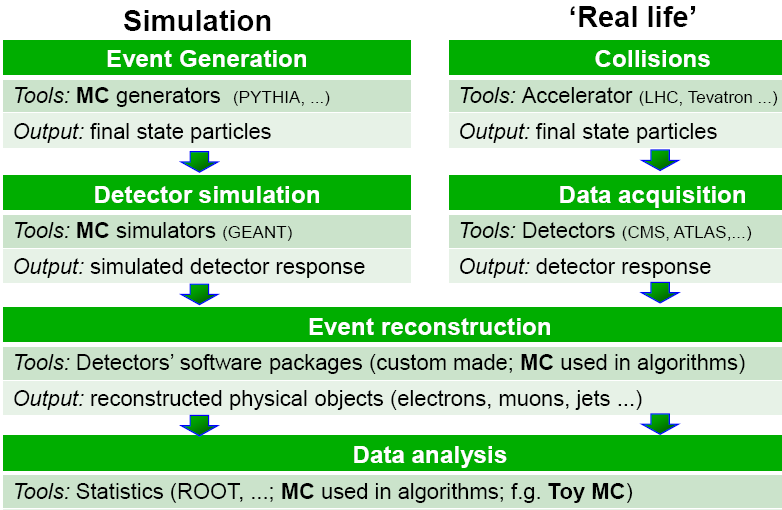
\includegraphics[scale = 0.7]{/home/anter/Desktop/Thesis/Figures/Simulation.png}\\
\vspace*{4mm} 
\caption{The comparison between Monte Carlo (MC) simulations generated by event generators and the real data produced by the particle collisions and observed in the detectors.}
\label{fig:sim}
\end{center}
\end{figure}

There are a variety of MC event generators which are commonly used in high energy physics. In this thesis, the three leading order (LO) generators : \PYTHIA, \MadGraphF and \HERWIG~as well as the next-to-leading order (NLO) generator \POWHEG are used. These generators are described one by one in the following sections.

\subsection{\PYTHIA}
\PYTHIA~is the most widely used program to generate the collisions at high energies for p-p, e-e and e-p colliders. It contains theoretical models for a number of physics processes which include hard and soft interactions, parton distribution functions, initial-state and final-state parton showers, multi-parton interactions, fragmentation and decay. It has a feature to interface with the external programs. It uses the Lund string hadronization model \cite{Lund} to describe the hadronization process. \PYTHIA~was originally coded in FORTRAN language under the version 6 i.e. \PYTHIAS \cite{Sjostrand:2006za}. In 2004, it was rewritten in C\plusn\plus and was released as \PYTHIAE \cite{Sjostrand:2007gs} in 2007. The two versions differ in the description of multi-parton interactions. Both the versions use LO calculations to derive the colored partons from the hard interaction which hadronize into colorless objects like hadrons. For the studies in this thesis, \PYTHIAS with tune \Ztwostar \cite{Field:2011iq} and \PYTHIAE with tunes CUETS1 and CUETM1 \cite{Khachatryan:2015pea} have been used. 

\subsection{\MadGraphF}
\MadGraphF~\cite{Alwall:2011uj} generates matrix elements for high energy physics processes, such as decays and $2 \rightarrow n$ scattering processes. The event information of the particles involved in the hard process such as particle ID, momenta, spin etc. is stored in the Les Houches format \cite{Alwall:2006yp} which can be interfaced to other generators. In the current study, \MadGraphF has been interfaced to \PYTHIAS with tune \Ztwostar to handle the rest of the generation steps which involve parton showering and hadronization. Matching algorithms make sure that no double-counting occurs between the tree-level and the parton-shower-model-generated partons. \MadGraphFn\plusn \PYTHIAS (\MGP) samples are used mainly for general comparisons to the data and calculating the detector resolution. 

\subsection{\HERWIG}
\HERWIG~(Hadron Emission Reactions With Interfering Gluons) \cite{Corcella:2000bw} is a multi-purpose event generator which performs the LO calculations. It uses angular ordering for parton showers and cluster model for hadronization. The hard lepton-lepton, lepton-hadron and hadron-hadron scattering as well as soft hadron-hadron processes can be simulated using \HERWIG~generator. This generator can be interfaced to external matrix element generators. \HERWIG~was written in FORTRAN language and a version in C\plusn\plusn is also available as \HERWIGPP \cite{Bahr:2008pv}. We have used the \HERWIGPP generator with the default tune of version 2.3 \cite{Bahr:2008tf} to generate the samples which have been used to study the non-perturbative effects. 

\subsection{\POWHEG}
\POWHEG (Positive Weight Hardest Emission Generator) generator performs the fixed NLO calculations merged with parton showers \cite{Frixione:2007vw, Nason:2004rx, Alioli:2010xa}. This generator used a computer framework known as \POWHEG BOX \cite{Oleari:2010nx} to implement NLO calculations in shower MC programs. It can be interfaced with all modern shower MC programs that support the Les Houches Interface format. It contains the hard matrix elements for NLO dijet production. \POWHEG has been interfaced to \PYTHIAE with tunes CUETS1 and CUETM1 to include the parton shower and hadronization, 
%The geometrical representation of detector elements focuses on the definition of solid models and their spatial position. 
\section{Detector Simulation}
The particles generated by MC event generators are passed through a computer program which does the detector simulation. It defines the detector system including its geometry, material and electronics properties. The detector simulation describes the nature of the interactions of the particles with the material of the detector. While propagating through the detector material, these particles are allowed to decay according to their known branching fractions and decay kinematics. The particles can interact with the detector material through several physical processes, including electron bremsstrahlung, energy loss by ionization, multiple scattering, hadron showering etc., which are simulated or parametrized in the corresponding parts of the detector. In CMS, the detector response is simulated by two approaches : \\ \newline
{\bf Full Simulation -} Full Simulation is based on a C\plusn\plus simulation toolkit \GEANTfour (GEometry ANd Tracking) \cite{Agostinelli:2002hh}. It is a successor of a FORTRAN based \GEANTthree and handles the interactions of particles with matter over a wide range of energy. In \GEANTfour, the uniform and non-uniform electromagnetic, magnetic and electric fields can be specified. The equation of motion of the particle in the field gives the track of the particle. A physical interaction of a track in the sensitive region of a detector is called a hit. The secondary particles produced are stored in a stack with the information of their kinematic properties as well as the vertex position where the interaction has occurred. A large number of MC events may have to be produced for a feasible physics analysis. The complete detector simulation of CMS using \GEANTfour is rather time consuming. So a Fast Simulation framework has been developed in the general software framework of the CMS for the fast simulation of the detector response.\\ \newline 
{\bf Fast Simulation -} In Fast Simulation \cite{Abdullin:2011zz}, detector effects are parametrized instead of simulating these from first principles as done in Full Simulation. In Fast Simulation package, the events are produced at much faster rates as compared to the Full Simulation package, while maintaining almost the same level of accuracy for physics studies. The format of the Fast Simulation data output is fully compatible with the standard Full Simulation one. 

After simulating the detector response, it is then transformed into a digital signal with the help of electronics and this step is called digitization. The simulated output of the detector response needs to be as close as possible to the real data coming from the CMS detector. After this, the event reconstruction algorithms are applied to both simulated and real events.
%A head-on collision between two protons taking place at very high energies can be visualized as an interaction between their constituent quarks and gluons. In a hard scattering process i.e. where the momentum transfer is large, the scattered partons fragment and hadronize into highly collimated bunches of particles. The showers of particles get deposited in the calorimeters in the form of conical structures called ``jets''.
\section{Event Reconstruction}
The aim of the event reconstruction is to identify the particles passing through the detector by interpreting the electrical signals produced in digitization. In event reconstruction, analysis-level objects are created by combining recorded signals from the tracker, calorimeters and muon detectors. Initially the reconstructed hits are collected which are combined to form tracks and calorimetric towers. Then higher level objects such as electrons, muons, photons and jets are reconstructed by combining the tracks and energy deposits. In CMS, all the particles are identified and reconstructed with a Particle Flow (PF) algorithm, discussed in detail in the next section.
%Each PFJet is matched to its corresponding GenJet topologically, by choosing the closest GenJet in $\eta$-$\phi$ plane. 

\subsection{Particle Flow Algorithm}
In the CMS, the identification and reconstruction of the particles is performed using the event reconstruction technique called Particle Flow (PF) algorithm \cite{CMS:2009nxa, CMS:2010byl}. %http://inspirehep.net/record/1324461.}
The PF algorithm combines the information from individual sub-detectors. The additional identification and reconstruction of the tracks enhances the reconstruction performance. These tracks are used to identify the primary vertices in an event. \\ \newline
{\bf Track Reconstruction -} The particles produced from the collisions leave the tracks in the sub-detectors as they traverse through the CMS detector. They follow helix paths due to presence of the strong magnetic field. An efficient tracking system is needed to measure momenta of the charged particles from the curvature of the tracks. The CMS uses an iterative tracking algorithm, the Combinatorial Track Finder (CTF) algorithm \cite{Adam:2005cg}, which first generates the track seeds by grouping the hits in the innermost layers. Then a pattern recognization is performed using a Kalman filter \cite{Fruhwirth:1987fm}, where hits coinciding with the predicted trajectory of the charged particle are found. Then the best parameters are estimated for all hits along the trajectory and fitting is performed. Finally, the quality criteria are applied to the tracks to reject the badly reconstructed ones and to decrease the fake rate, defined as the ratio between fake tracks and all tracks. These all steps are performed iteratively which are ordered by the level of difficulty in identifying the
tracks. \\ \newline
{\bf Primary Vertex Reconstruction -} The increasing center-of-mass energy and instantaneous luminosity enhances the probabilities of multiple pp collisions per bunch crossing as well occurrence of two or more hard interactions between partons in the same pp collisions giving rise to pileup events. Hence, the identification of the primary vertex of the main hard interaction becomes important. The CMS performs the primary vertex reconstruction in two steps : First, a set of promptly produced tracks are selected and grouped together in clusters, using a deterministic annealing (DA) algorithm \cite{KRose}. The tracks are grouped based on their $z$-coordinate at the point of closest approach to the beam line. For each track, the $z$-coordinate of the point of closest approach to the beam-line is referred as $z_i$ with associated uncertainty as $\sigma_i$. These tracks must be assigned to an unknown number of vertices denoted by a $z$-coordinate of $z_k$. If a track is assigned to only one vertex, it is referred as a hard assignment. It is represented by values of probability $p_{ik}$ = 1 if track $i$ is assigned to vertex $k$ and 0 otherwise. For the soft assignments, the tracks can be associated with more than one vertex such that $p_{ik}$ has value between 0 and 1 representing the probability of the assignment of track $i$ to vertex $k$ in a large ensemble of possible assignments. \chisq is defined as :
\begin{equation}
\chisq = \sum\limits_{ik}^{} p_{ik} \frac{(z_i - z_k)^2}{\sigma^2_i} 
\end{equation} 
Instead of minimizing the \chisq, the DA algorithm finds the most likely distribution for a given value $\chi_{0}^{2}$ which is then decreased until it finds a good reliable minimum. Once the tracks are assigned to the different vertices, a three dimensional fitting is done using the adaptive vertex fitter \cite{Fruhwirth:2007hz} where each track is assigned a weight ($w$) between 0 and 1. After fitting, the tracks are labelled as either good with $w$ = 1 or outliers with $w$ value close to 0. The sum of these weights gives a rough estimate of the number of tracks associated with the vertex. The number of degrees of freedom in a fit is given by \ndof = 2$\sum\limits_i w_i$ - 3, where $w_i$ is the weight of the $i$th track and the sum runs over all tracks associated with the vertex. The vertices having \ndof \gr 4 i.e. having at least four tracks assigned to each vertex, are considered. All the reconstructed vertices are ordered by the sum of the squared track momenta $\sum p^2_{\rm T}$ and the one having largest sum is selected as the primary vertex of interest.

The PF algorithm works independently of the vertex reconstruction. The PF event reconstruction algorithm basically converts the detector signals back to physical objects by using PF event reconstruction algorithm which is illustrated in Fig.~\ref{fig:PF_algo}. The transverse momenta of the final state stable particles or energies of the calorimeter towers are taken as the inputs to the PF algorithm. The PF algorithm first collects the reconstructed hits in each sub-detector independently and creates a list of reconstructed elements (referred as blocks) which consists of charged tracks in tracker, energy clusters in calorimeters and muon tracks in muon system. Then a link algorithm connects topologically compatible blocks producing PF objects. The PF objects consist of all stable particles : electrons, muons, photons, charged and neutral hadrons. The energy of the the electrons is determined from the track momentum at the main interaction vertex along with the corresponding ECAL energy deposits and the energy sum of all bremsstrahlung photons associated with the tracks. 
\begin{figure}[!t]
 \begin{center}
 \vspace*{4mm} 
 %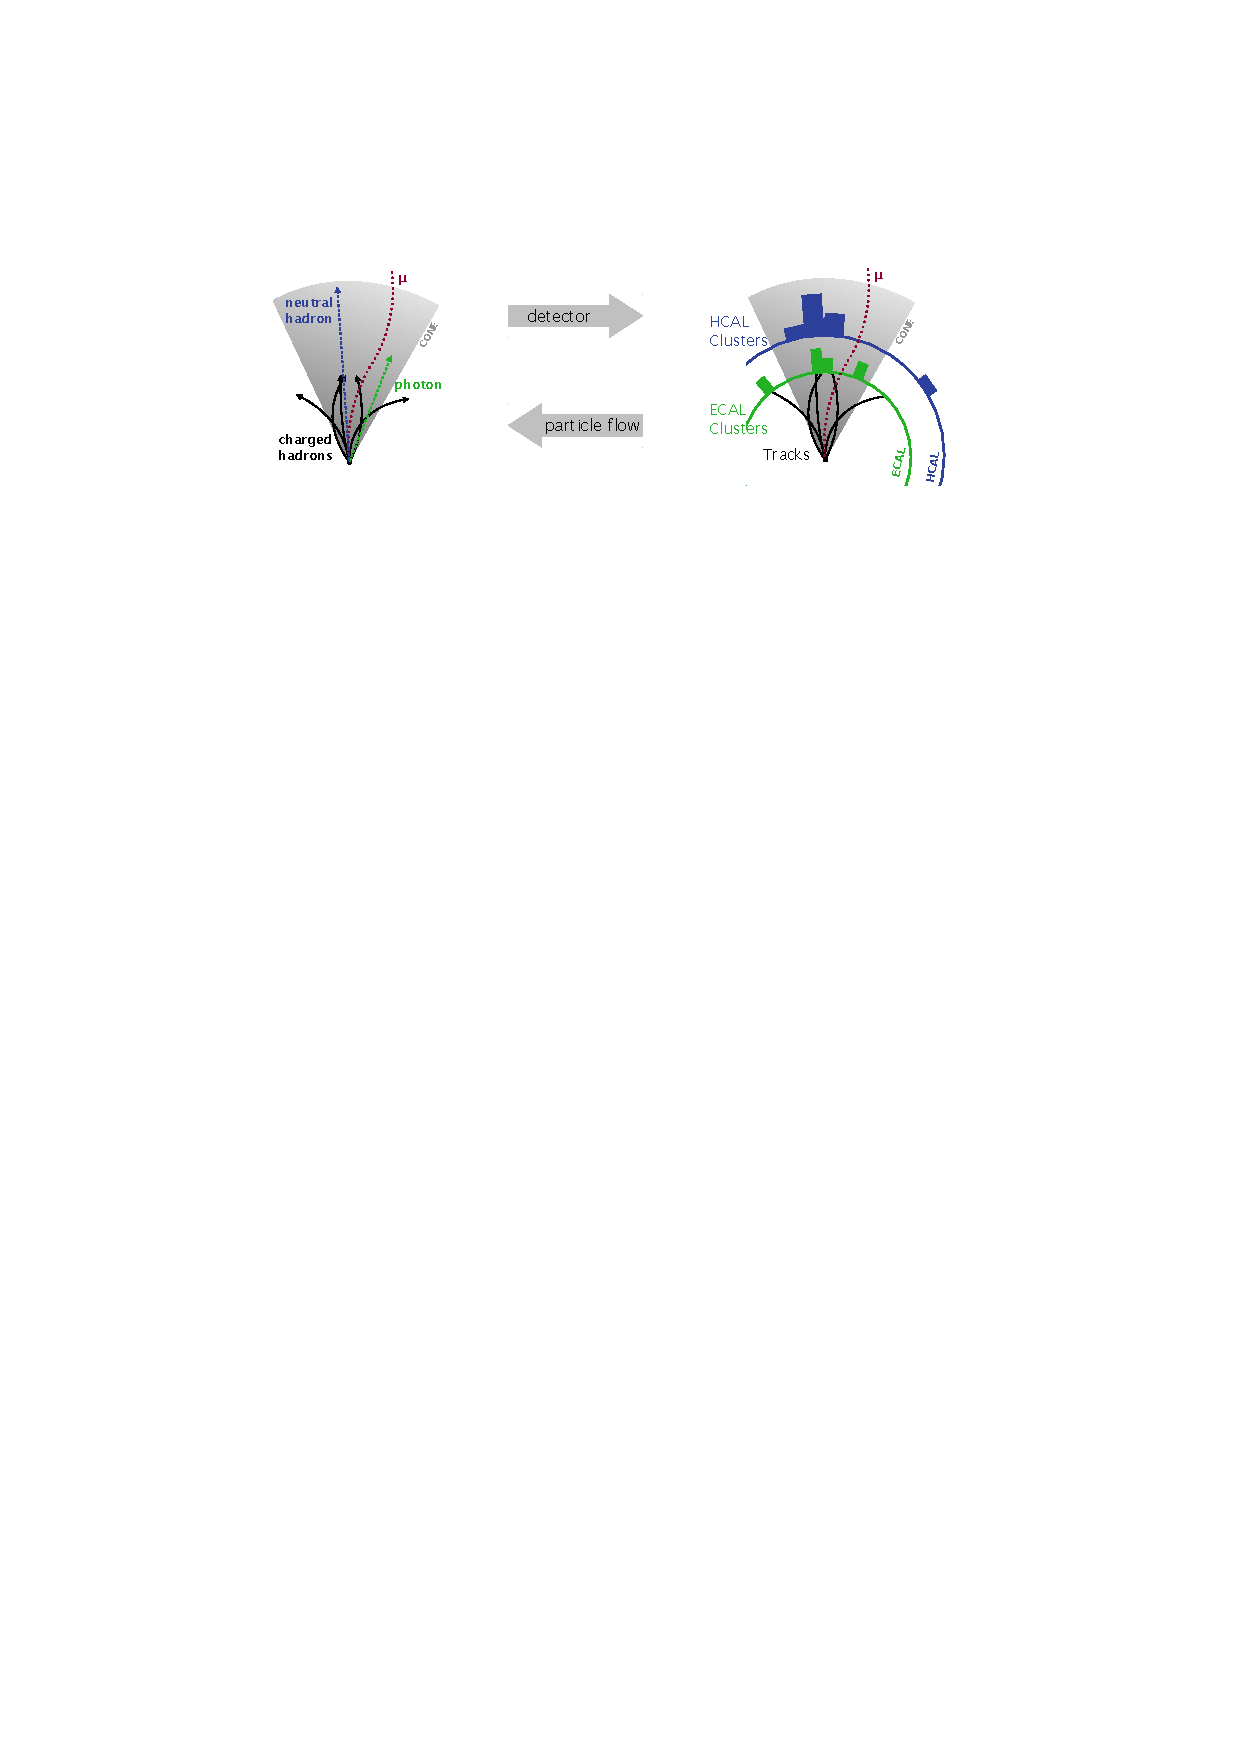
\includegraphics[width=1.\textwidth]{/home/anter/Desktop/Thesis/Figures/cropped_PF.pdf}
 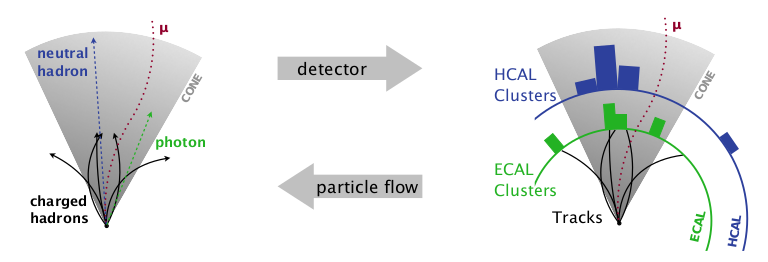
\includegraphics[width=1.\textwidth]{/home/anter/Desktop/Thesis/Figures/Final/PF.png}
 \vspace*{5mm}
 \caption[The Particle Flow (PF) algorithm is used by the CMS to identify and reconstruct the particles. The PF converts the sub-detector measurements back to physical particle objects.]{The Particle Flow (PF) algorithm is used by the CMS to identify and reconstruct the particles. The PF converts the sub-detector measurements back to physical particle objects. Taken from \cite{Rabbertz:2017ssq}.}
 \label{fig:PF_algo}
 \end{center}
\end{figure}
The curvature of the tracks in tracker and muon chamber is used to estimate the energy of muons. The energy of photons is obtained directly from the ECAL measurement, corrected for zero-suppression effects\footnote{To suppress noise in the calorimeters, only cells with energies above a given threshold are considered and this procedure is known as zero-suppression.}. The energy of charged hadrons is calculated by combining the track momentum and corresponding energy clusters in ECAL and HCAL, corrected for zero-suppression effects as well as calibrated for the nonlinear response of the calorimeters. The energy of neutral hadrons is obtained from the corresponding calibrated ECAL and HCAL energies only. Along with the reconstruction of the PF objects, missing transverse energy (\ETmiss) is also determined using PF algorithm. \ETmiss is defined as the negative vector sum of transverse momenta (\pt) of all the isolated stable particles reconstructed in an event i.e. \ETmiss = $-\sum\limits_{\rm i}^{}\overrightarrow{p_{\rm T,i}}$. To avoid any kind of double-counting of energy, blocks of all PF reconstructed particle objects are removed and the energy of the calorimeter clusters is recalculated. Finally, the collection of PF objects is used to reconstruct the jets by using the different jet clustering algorithms. The jets are collimated sprays of hadrons and other particles produced by the hadronization of the quarks or gluons. The detailed description of jets is given in Sec.~\ref{sec:jets}. The jet algorithms, discussed in Sec.~\ref{sec:jet_algos}, are used for clustering of stable partons, particles or reconstructed particles. The jets are formed at different levels : parton level, particle level and detector or reconstructed level, as illustrated in Fig.~\ref{fig:jets}. In the CMS detector, jets are the localized deposits of energy in the calorimeter cells along with the large number of tracks in the direction of the deposited energy. The typical jet energy fractions contributed by charged particles, photons and neutral hadrons are
65\%, 25\% and 10\%, respectively. So, the PF algorithm reconstructs about 90\% of the jet constituents with good precision, whereas only 10\% depend on the less accurate response of the HCAL. Depending on the type of input to the jet algorithm, jets can be categorized into following different types :\\ \newline 
{\bf Generator Jets -} The stable particles generated by the MC event generators are clustered into generator jets (GenJets). At this particle level, the passage through the detector simulation has not been carried out. The objects at this level are photons, charged and neutral hadrons. Since the energy of GenJets is independent of the detector response, these are considered as reference objects for estimating the jet energy corrections, discussed in Sec.~\ref{sec:jet_corrections}. \\ \newline
{\bf Calorimetric Jets -} The Calometric jets (CaloJets) are reconstructed by taking the energy clusters deposited in the ECAL and HCAL calorimeter towers as inputs. One calorimetric tower consists of one HCAL cell surrounded by an array of 5 $\times$ 5 ECAL cells. The tower’s four-momenta are computed by taking the direction from the interaction point to the tower center. All towers with a transverse energy measurement above 300 MeV are considered in the clustering process. CaloJets are relatively simple objects because only calorimeter information is deployed, but they are strongly affected by the non-linearity of the calorimeter response. \begin{figure}[!h]
\begin{center}
\vspace*{3mm} 
\hspace*{-5mm}
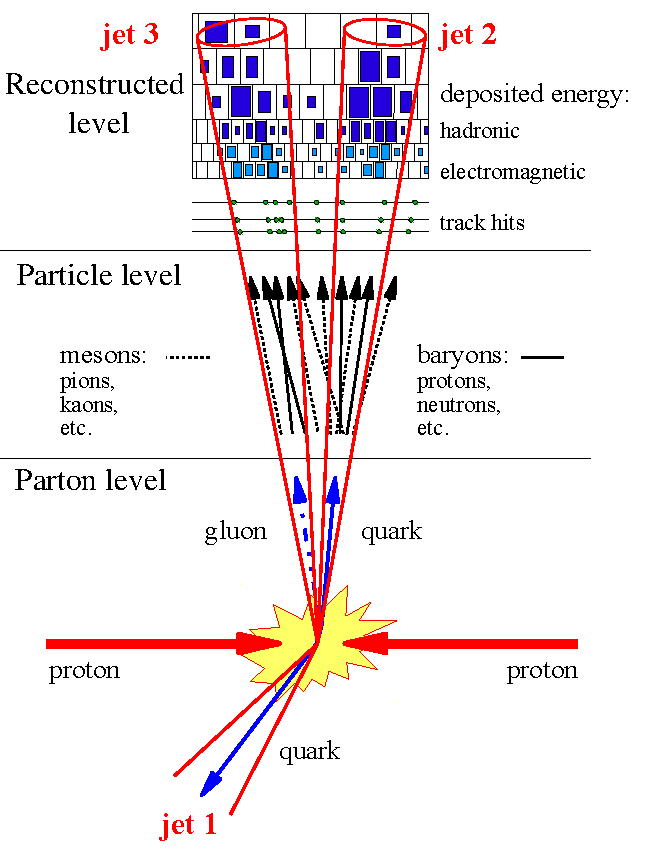
\includegraphics[scale = 0.95]{/home/anter/Desktop/Thesis/Figures/jet_levels_en_edited.pdf}\\
\vspace*{4mm}
\caption[Formation of jets in a proton-proton collision at different levels.]{In a proton-proton collision, the hard scattered quarks and gluons fragment to produce the showers of partons which get clustered into parton jets. The produced partons undergo hadronization and produce hadrons which form particle jets. The hadrons deposit their energies into the calorimeters in the form of reconstructed jets. Taken from \cite{Schorner-Sadenius:2015cga}.}
\label{fig:jets}
\end{center}
\end{figure} Since the readout of calorimeter measurements is fast, CaloJets are commonly used by the trigger system. \\ \newline
{\bf Particle Flow Jets -} The clustering of particle flow candidates give detector level jets called Particle Flow jets (PFJets). The four-momenta of the particles is taken as the input. The use of the tracker system and high granularity of the ECAL gives better energy resolution calculated using the independent measurements of charged hadrons and photons clustered to form a jet. Hence PFJets perform better than CaloJets and are the standard jets used at CMS.

We the study of the jets formed by clustering the particle flow candidates using the anti-\kt algorithm with a jet size parameter of $R$ = 0.7. 

\subsection{Jet Energy Corrections}
\label{sec:jet_corrections}
The measured energy of jets cannot be directly translated to the energy at true particle or parton level. This is because of the nonlinear and nonuniform response of the calorimeters, effects of pileup and small residual effects in the data remaining after the corrections based on MC simulations. Hence the jet energy corrections (JEC) \cite{Chatrchyan:2011ds, Khachatryan:2016kdb} are used to correct the measured jet energy and relate it to the corresponding true particle jet energy. To correct the energy of jets, the CMS follows a factorized approach, as presented in Fig.~\ref{fig:jec}, where JEC are applied in a sequential manner with fixed order, i.e. the output of one step serves as the input for the next one. Each level of correction takes care of a different effect and is independent of each other. At each step, the jet four-momenta is scaled with a correction factor which depends on jet \pt, $\eta$, flavor etc.

\begin{figure}[!h]
 \begin{center}
 \vspace*{4mm} 
 \hspace*{-11mm}
 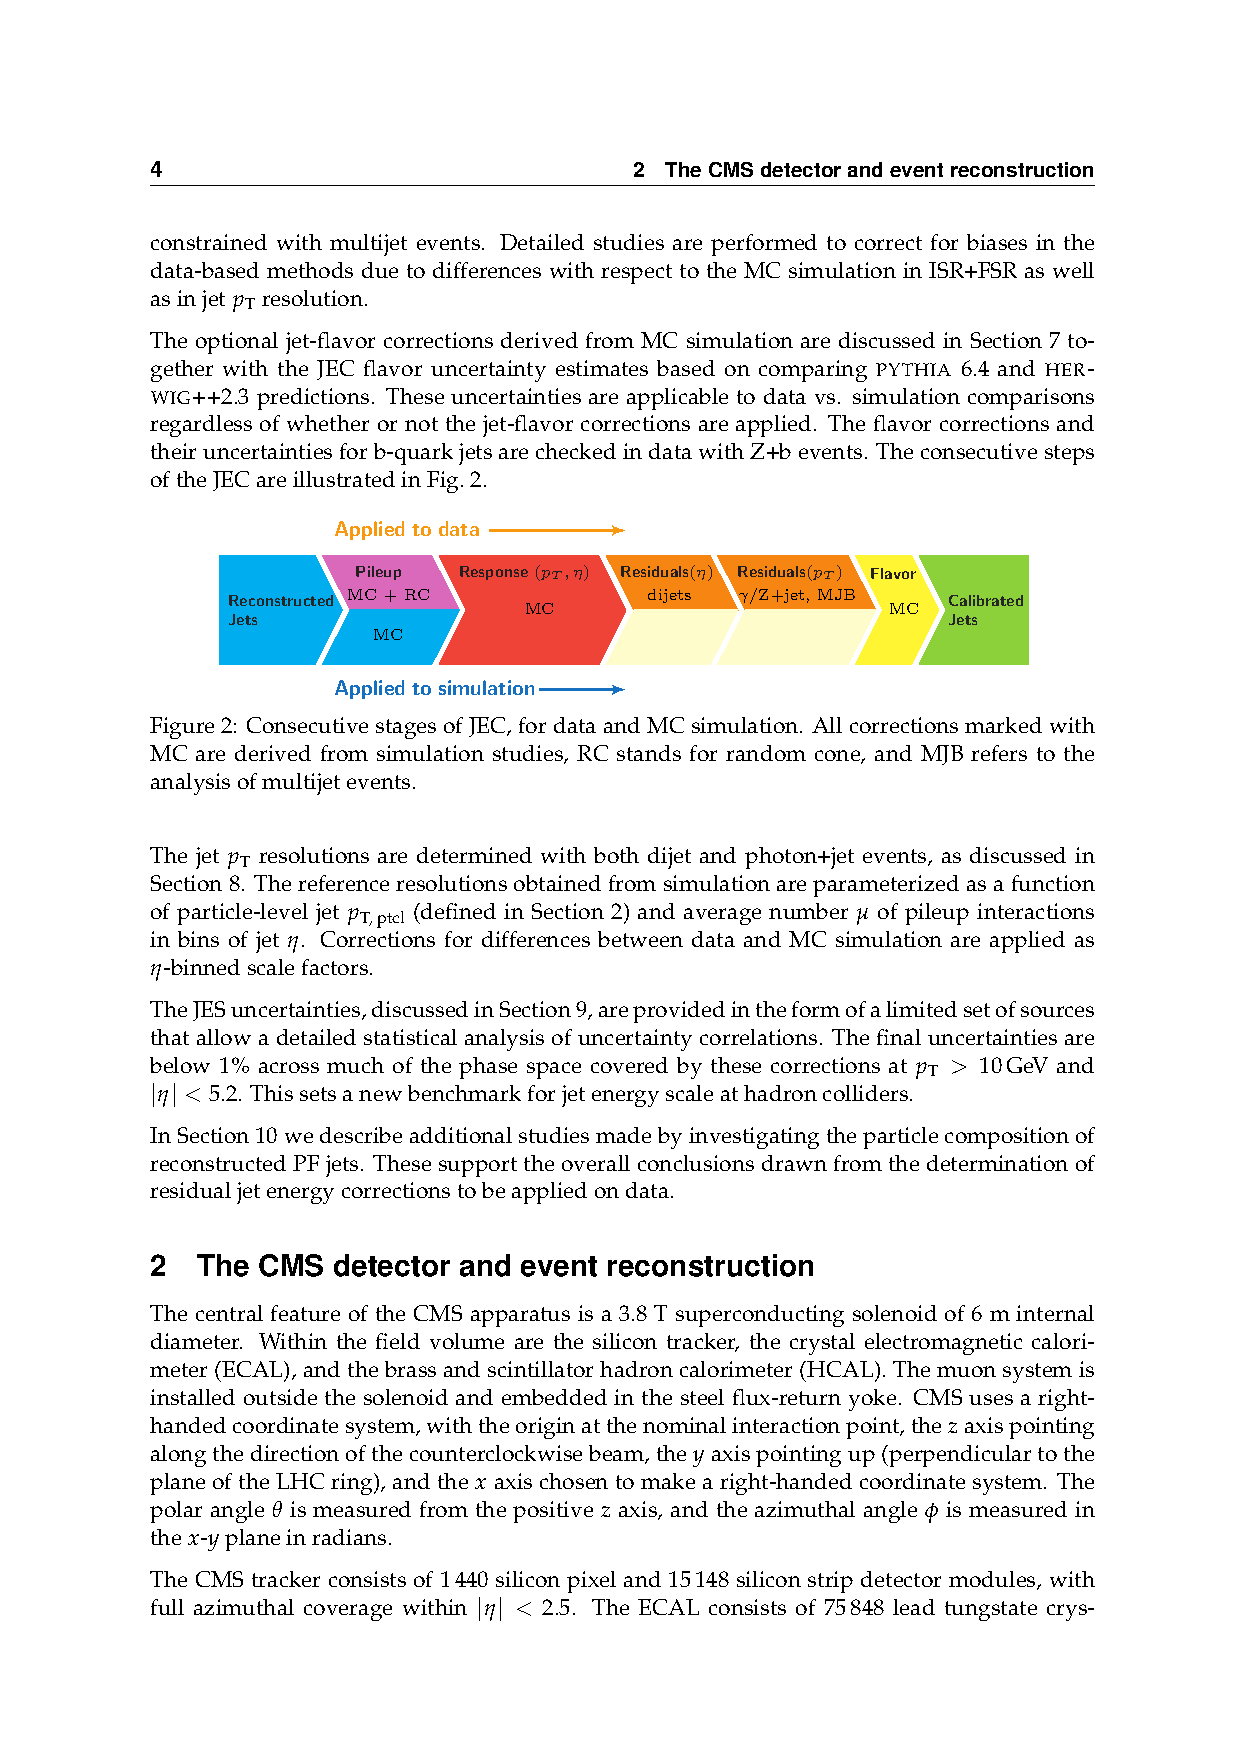
\includegraphics[width=1.3\textwidth]{/home/anter/Desktop/Thesis/Figures/New/JEC.pdf}\\
 \vspace*{5mm}
 \caption[A schematic diagram of the factorized jet energy corrections (JEC).]{A schematic diagram of the factorized jet energy corrections (JEC) applied to the data (upper half) and simulation (lower half). The reconstructed jets are corrected for pileup effects, non-uniform \pt and $\eta$ response and residual differences between the data and Monte Carlo simulations along with optional flavor corrections. All corrections marked with MC are derived from simulation studies, RC stands for random cone, and MJB refers to the analysis of multijet events. Taken from \cite{Khachatryan:2016kdb}.}
 \label{fig:jec}
 \end{center}
\end{figure}

The corrected jet transverse momentum $p^{\rm corr}_{\rm T}$ is obtained by applying all correction factors subsequently on raw or uncorrected jet transverse momentum $p^{\rm raw}_{\rm T}$ as below :

\begin{equation}
p^{\rm corr}_{\rm T} = c_{\rm res}(\eta,p''_{\rm T})\cdot c_{\rm mc}(\eta,p'_{\rm T})\cdot c_{\rm pileup}(\eta,\rho,{\rm A}_{j},p^{\rm raw}_{\rm T})\cdot p^{\rm raw}_{\rm T}
\end{equation}
where $p'_{\rm T}$ is the transverse momentum obtained after applying the pileup correction factor $c_{\rm pileup}$ on $p^{\rm raw}_{\rm T}$, $p''_{\rm T}$ is the transverse momentum obtained after applying the additional correction factor $c_{\rm mc}$ because of relative and absolute effects derived from MC. Finally, a correction factor $c_{\rm res}$ is applied for residual effects derived from the data. The corrections applied at each step are discussed below : \\
{\bf Pileup Corrections -} The additional proton-proton collisions occur within the same bunch-crossing along with the main hard interaction and give rise to pileup events. The particles produced from the pileup events get clustered into the jets coming from the hard interaction and increase the jet energy. This extra energy needs to be subtracted from the reconstructed jet energy. This is done by applying the pileup corrections to raw jet $p^{\rm raw}_{\rm T}$. The pileup corrections are determined by simulating a sample of QCD dijet events with and without pileup effects. The pileup correction factor, $c_{\rm pileup}$ is calculated from jet area method using the pileup density $\rho$ in the event and the jet area ${\rm A}_{j}$. $c_{\rm pileup}$ is parametrized as a function of $\rho$, ${\rm A}_{j}$, jet \pt and $\eta$. There are corrections for residual differences between the data and detector simulation which are determined using the random cone (RC) method in zero-bias events. Hence the different pileup corrections are applied to the data and the MC simulations. \\ \newline
{\bf MC Corrections -} The next correction applied to the pileup corrected jets is based on MC simulated QCD events. Due to the inefficiencies introduced by the detector simulation, the reconstructed jet \pt is not the same as that of the generated one. This difference is corrected with the factor, $c_{\rm mc}$ which is derived by comparing the measured jet \pt to the particle level jet \pt. The corrections are determined as a function of jet \pt and $\eta$ which make the detector response uniform over these two variables. \\ \newline
{\bf Residual Data Corrections -} The jets corrected with above mentioned corrections are further corrected for remaining small differences between the data and MC simulations. This correction is applied only to the data. The correction factor $c_{\rm res}$ is derived using data-driven methods. The relative residual corrections are evaluated using dijet events in which a probe jet is calibrated using a tag jet. The last correction applied is the absolute residual correction in which the precisely reconstructed $Z$ bosons balanced to a jet are used to calibrate the jet energy. \\ \newline
{\bf Flavor Corrections -} These corrections correct the jets for flavor dependence (b, $\tau$ etc.) and are optional. These are extracted using Z\plusn jet and photon\plusn jets simulated events. %The flavor corrections have not been applied for 8 TeV CMS data.

The process of correction of jets by using JEC introduces uncertainties in the final corrected jet energy which are discussed in Sec.~\ref{sec:jecs_unc}. After correcting the jets, the multijet event cross-sections are measured which are discussed in the following chapter.
